\documentclass{article}

\usepackage[english]{babel}
\usepackage[utf8]{inputenc}
\usepackage{amsmath,amssymb}
\usepackage{parskip}
\usepackage{graphicx}
\usepackage{listings}
\usepackage{subfig}
\usepackage{float}
\lstset{
    numbers=left, 
    numberstyle= \tiny, 
    keywordstyle= \color{ blue!70},
    commentstyle= \color{red!50!green!50!blue!50}, 
    frame=shadowbox, % 阴影效果
    rulesepcolor= \color{ red!20!green!20!blue!20} ,
    escapeinside=``, % 英文分号中可写入中文
    xleftmargin=2em,xrightmargin=2em, aboveskip=1em,
    framexleftmargin=2em,
    breaklines=true,
    language=R
} 

% Margins
\usepackage[top=2.5cm, left=3cm, right=3cm, bottom=4.0cm]{geometry}
% Colour table cells
\usepackage[table]{xcolor}

% Get larger line spacing in table
\newcommand{\tablespace}{\\[1.25mm]}
\newcommand\Tstrut{\rule{0pt}{2.6ex}}         % = `top' strut
\newcommand\tstrut{\rule{0pt}{2.0ex}}         % = `top' strut
\newcommand\Bstrut{\rule[-0.9ex]{0pt}{0pt}}   % = `bottom' strut

%%%%%%%%%%%%%%%%%
%     Title     %
%%%%%%%%%%%%%%%%%
\title{CSCI946 Assignment}
\author{Yao Xiao \\ SID 2019180015}
\date{\today}

\begin{document}
\maketitle

%%%%%%%%%%%%%%%%%
%   Problem 1   %
%%%%%%%%%%%%%%%%%
\section{Describe this MNIST data set and its training and test subsets.}
The MNIST database of handwritten digits consists of a training set of 60,000 examples, and a test set of 10,000 examples. 
The training set and test set are collected from 250 different people's handwritten numbers.
It is a subset of a larger set available from NIST. Additionally, the black and white images from NIST were size-normalized and centered to fit into a 28x28 pixel bounding box and anti-aliased, which introduced grayscale levels.

\section{Describe how you reshape each image into a long vector and how you train the LRC or SVM.}
First use numpy vectors to represent image data. The image data is grayed out and then stored in a numpy array. At this time, the value of each element is between 0 and 255. Next, we convert it to grayscale, map it to the range of 0 to 1, round each element to make its value 0 or 1, and then convert it to a binary matrix. Finally, convert the 20 x 20 binary matrix into a 28 x 28 vector.

\begin{lstlisting}
    def convert2vec(image):
        img = Image.open(image).convert('L')
        arr_img = np.arry(img, 'i')
        img_normlization = np.round(arr_img / 255)
        img_arr = np.reshape(img_normlization, (1, -1))
\end{lstlisting}

However, in our project, we can directly load the data using the set image input size. Using LRC model training, we can obtain better classification accuracy by adjusting the parameters multiple times.
\begin{lstlisting}
input_size = 784
num_classes = 10
num_epochs = 50 
batch_size = 64
learning_rate = 0.01

train_dataset = dsets.MNIST(root='mnist',
                            train=True,
                            transform=transforms.ToTensor(),
                            download=True)
test_dataset = dsets.MNIST(root='mnist',
                           train=False,
                           transform=transforms.ToTensor(),
                           download=True)

# Data loader
train_loader = torch.utils.data.DataLoader(dataset=train_dataset,
                                           batch_size=batch_size,
                                           shuffle=True)
test_loader = torch.utils.data.DataLoader(dataset=test_dataset,
                                          batch_size=batch_size,
                                          shuffle=True)

# LRC model
model = nn.Linear(input_size, num_classes).cuda()
\end{lstlisting}

\section{Describe how you designed your CNN, justify your approach, and describe how you trained it. Explain
which other settings of the network parameters and/or training parameters that you tried, and describe the
changes on classification accuracy and training time.}

\begin{figure}[H]
    \caption{Structure of LeNet}
    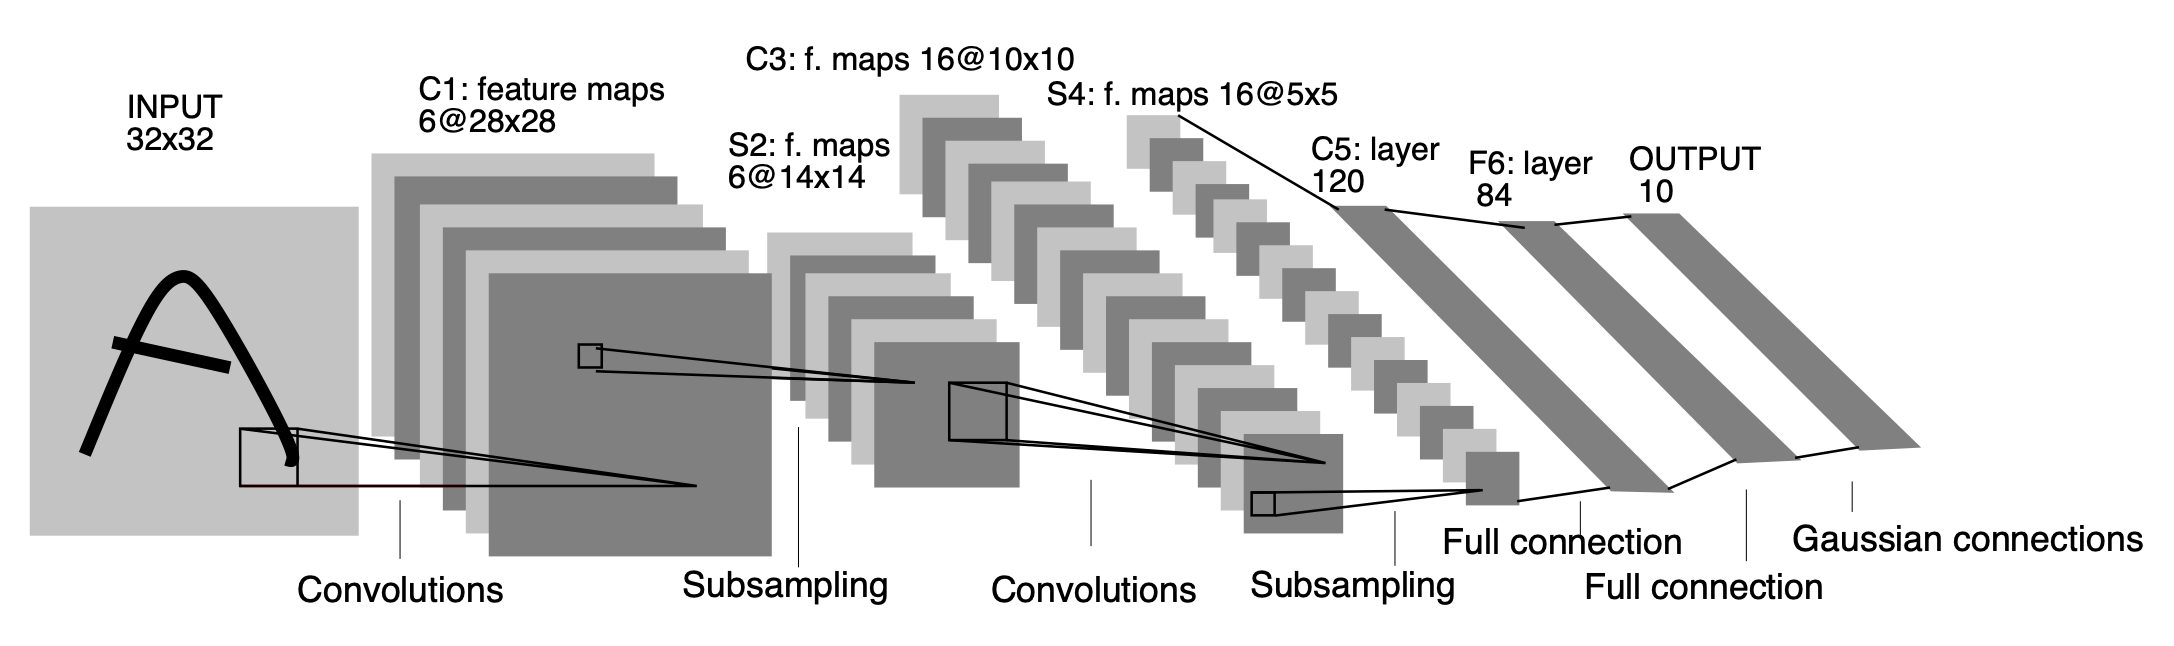
\includegraphics[width=1\textwidth]{Fig1}
\end{figure}

​LeNet is the most classic convolutional neural network designed for handwritten digit recognition, and is known as one of the most representative experimental systems in the early convolutional neural networks.
LeNet uses convolution, parameter sharing, pooling and other operations to extract features through clever design, avoiding a large amount of computational cost, and finally uses a fully connected neural network for classification and recognition. This network is also the starting point of a large number of neural network architectures recently.
The LeNet model has 8 layers, Input 32*32 handwritten font pictures, these handwritten fonts contain 0-9 numbers, which is equivalent to 10 categories of pictures, and output the classification results, a number between 0-9.

\textbf{For the LRC model:}

In this model, there are there main attributes adjusted: learning rate, batch size and epoch times.

The experiment 1 settings: $lr=0.1$, $batch size=32$, $epoch=20$:
\begin{figure}[H]
    \centering
    \caption{EXP1 for LRC}
    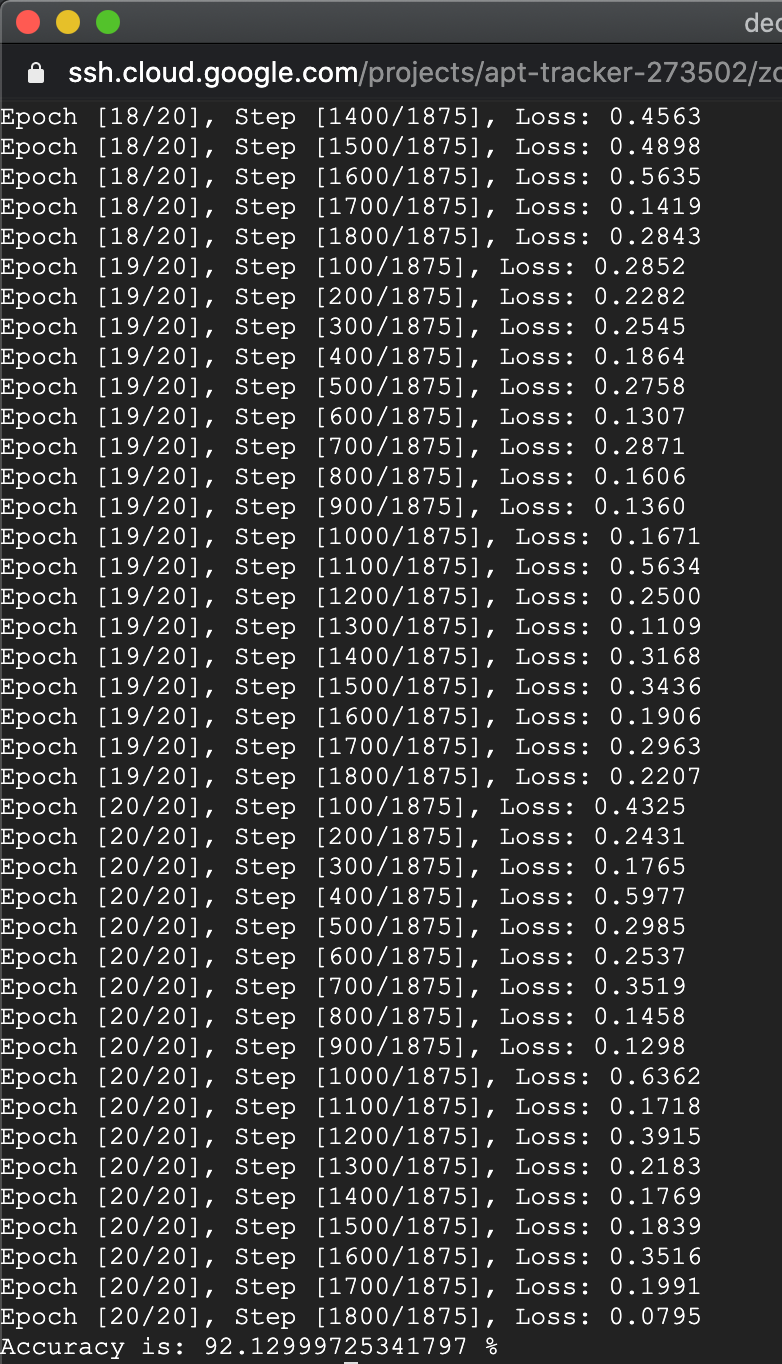
\includegraphics[width=0.28\textwidth]{lrc_1}
\end{figure}

The experiment 2 settings: $lr=0.3$, $batch size=64$, $epoch=20$:
\begin{figure}[H]
    \centering
    \caption{EXP2 for LRC}
    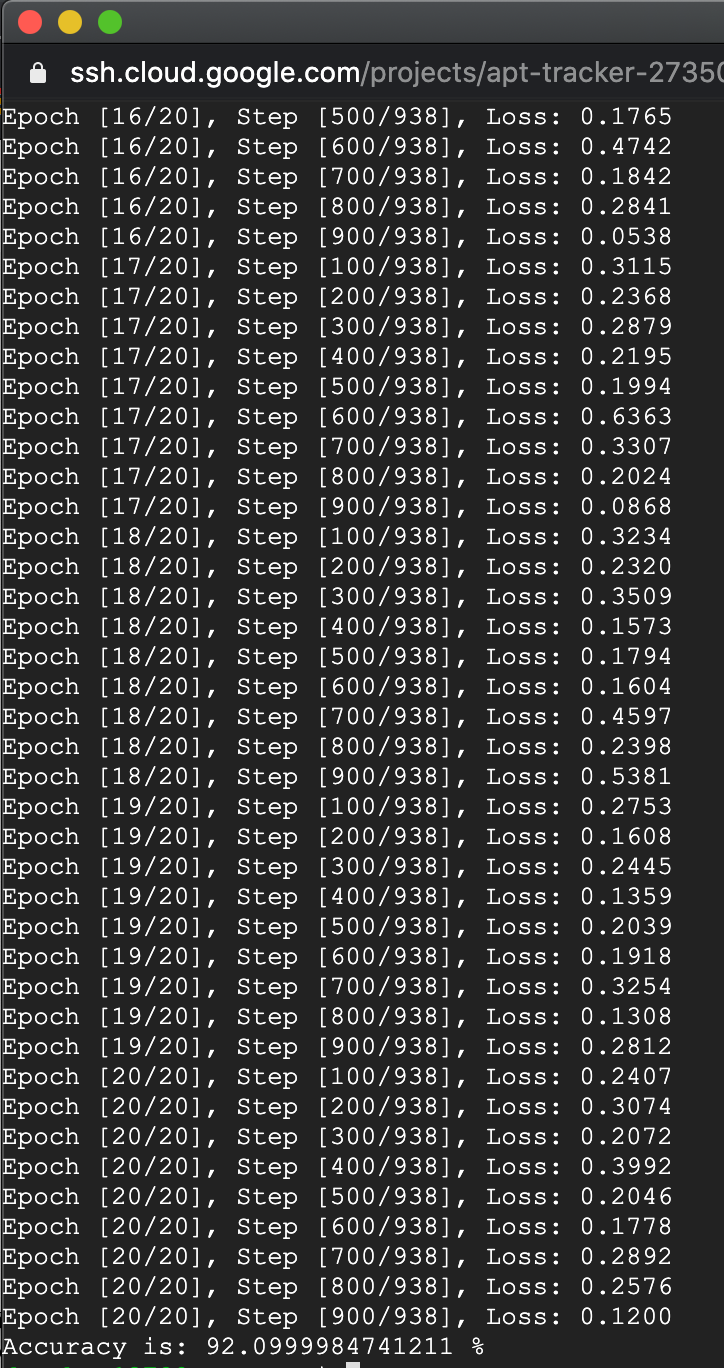
\includegraphics[width=0.28\textwidth]{lrc_2}
\end{figure}

The experiment 3 settings: $lr=0.1$, $batch size=128$, $epoch=40$:
\begin{figure}[H]
    \centering
    \caption{EXP3 for LRC}
    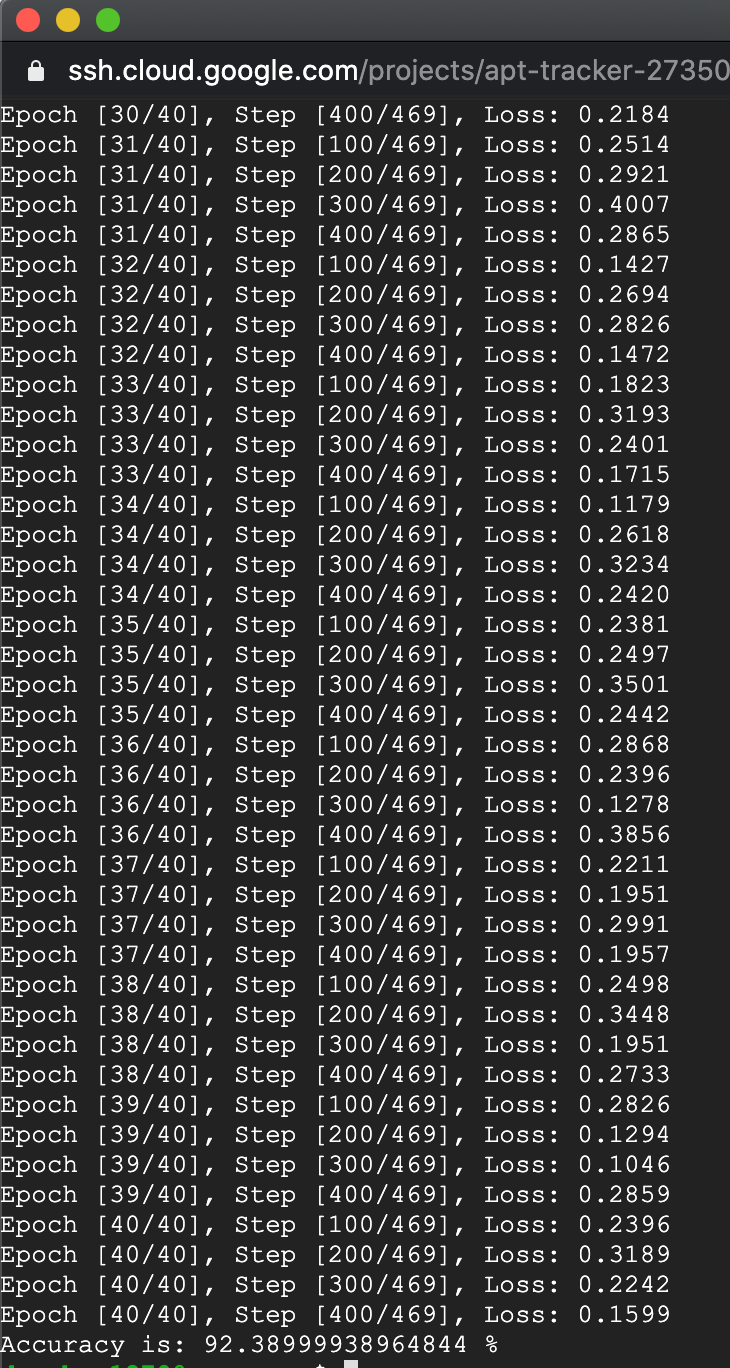
\includegraphics[width=0.28\textwidth]{lrc_3}
\end{figure}

The experiment 4 settings: $lr=0.5$, $batch size=128$, $epoch=40$:
\begin{figure}[H]
    \centering
    \caption{EXP4 for LRC}
    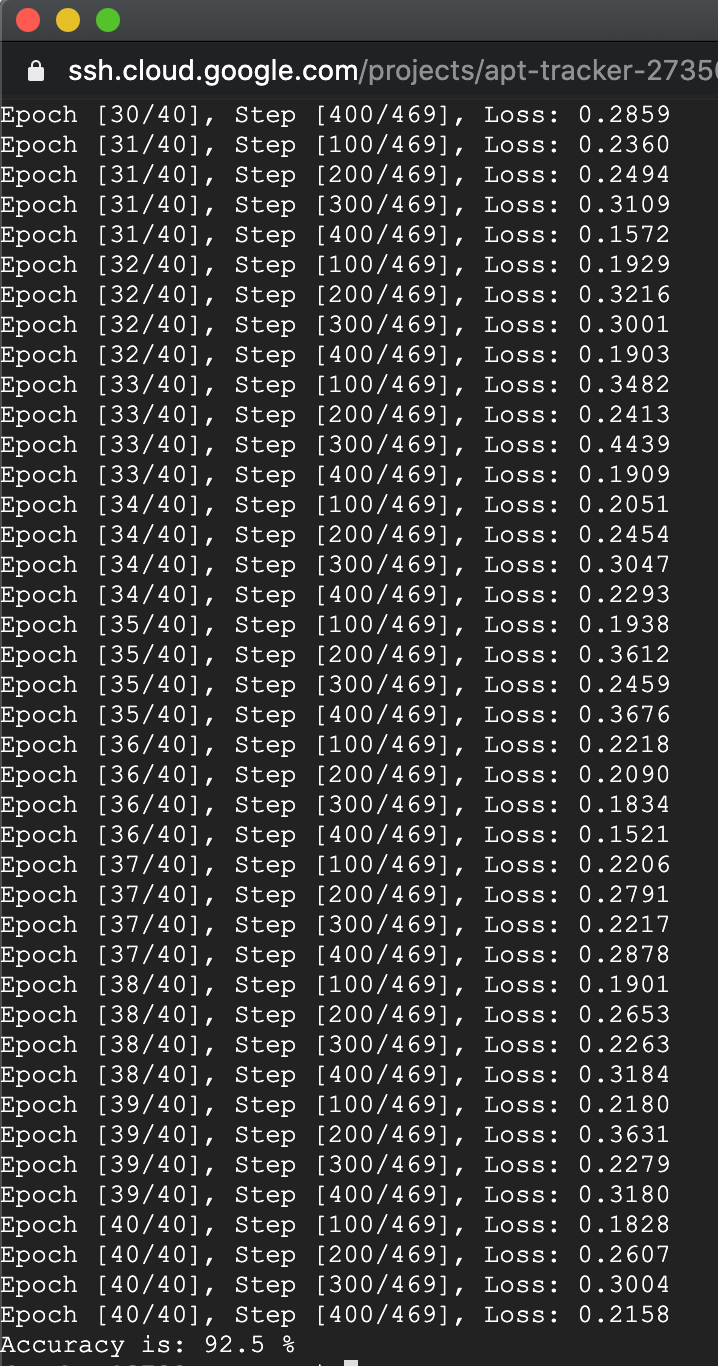
\includegraphics[width=0.28\textwidth]{lrc_4}
\end{figure}

\textbf{For the base LeNet model:}

In this model, there are there main attributes adjusted: batch size and epoch times.

The experiment 1 settings: $batch size=16$, $epoch=5$:
\begin{figure}[H]
    \centering
    \caption{EXP1 for LeNet}
    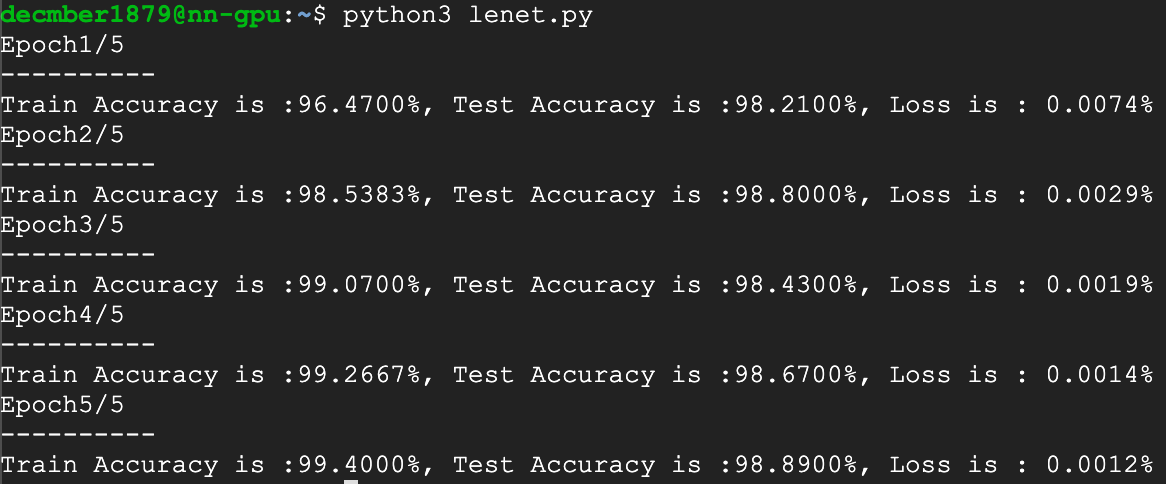
\includegraphics[width=0.6\textwidth]{lenet_1}
\end{figure}

The experiment 2 settings: $batch size=32$, $epoch=10$:
\begin{figure}[H]
    \caption{EXP2 for LeNet}
    \centering
    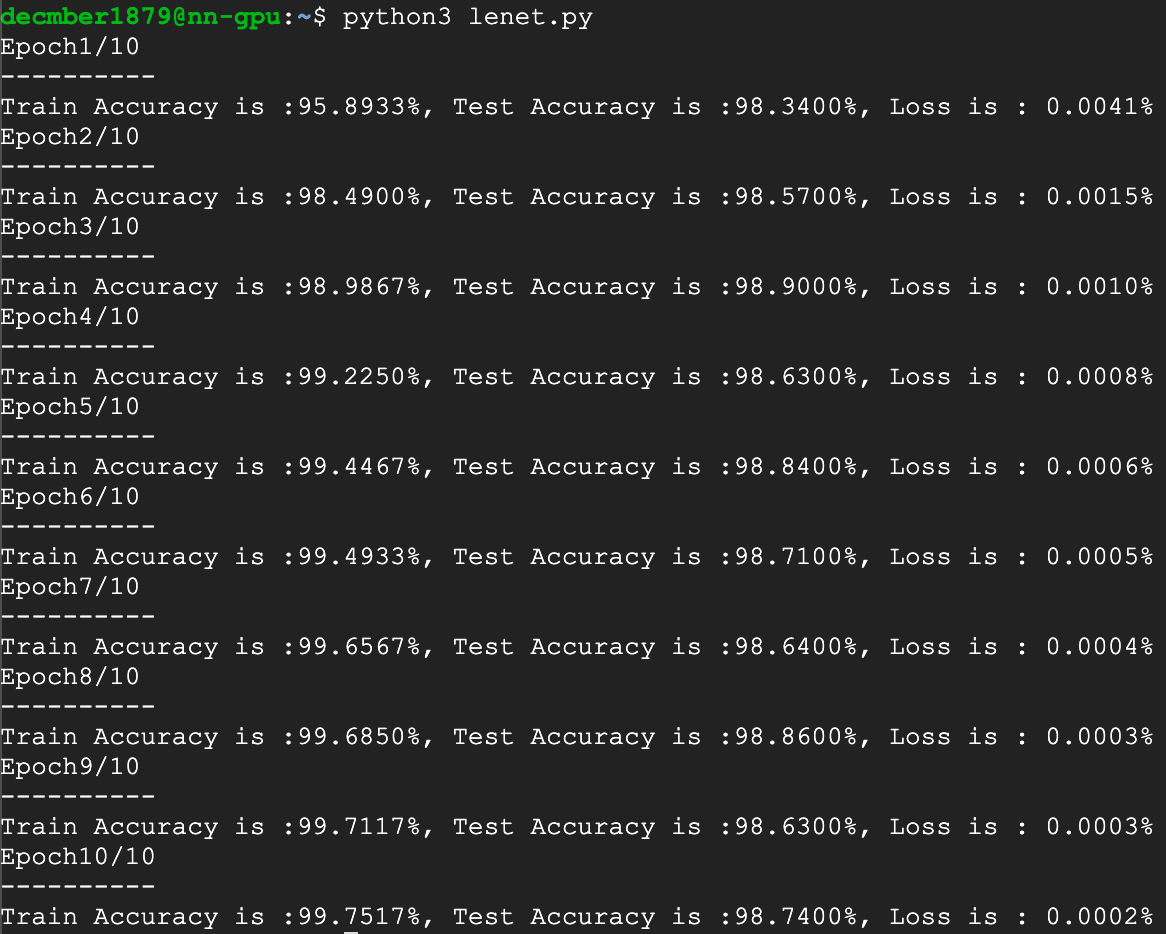
\includegraphics[width=0.6\textwidth]{lenet_2}
\end{figure}

The experiment 3 settings: $batch size=64$, $epoch=20$:
\begin{figure}[H]
    \caption{EXP3 for LeNet}
    \centering
    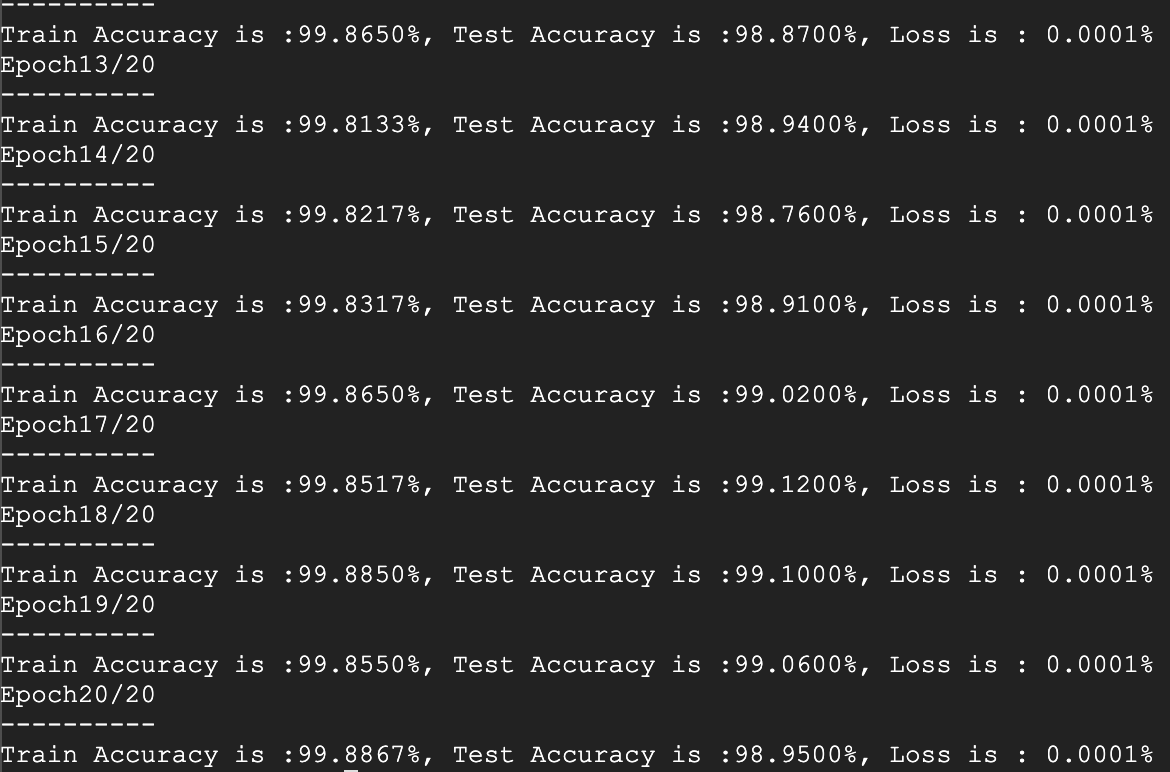
\includegraphics[width=0.6\textwidth]{lenet_3}
\end{figure}



\section{Report the best classification accuracy and the corresponding confusion matrices obtained by the
classification methods (LRC, SVM, and the CNNs). Evaluate and compare the classification performances.
Analyse and explain the results.}

We can see the above, the best accuracy result of LRC model is: 92.5\%,
in addition, the adjustment results of each round are improved, and EXP1 can obtain the lowest loss value.

The best accuracy result of LeNet model is: 98.95\%, although there are fluctuations, with the increase of batch sizh and epoch time, the result has also increased correspondingly, and the loss value has also achieved the lowest.

In summary, the larger the batch size and epoch time, the better the performance of CNN.
\section{Source Code}
\begin{lstlisting}
# Code for LRC
import torch
import torch.nn as nn
import torchvision.datasets as dsets
import torchvision.transforms as transforms
from torch.autograd import Variable

device = 0 if torch.cuda.is_available() else 'cpu'

input_size = 784
num_classes = 10
num_epochs = 50 
batch_size = 64
learning_rate = 0.01

train_dataset = dsets.MNIST(root='mnist',
                            train=True,
                            transform=transforms.ToTensor(),
                            download=True)
test_dataset = dsets.MNIST(root='mnist',
                           train=False,
                           transform=transforms.ToTensor(),
                           download=True)

# Data loader
train_loader = torch.utils.data.DataLoader(dataset=train_dataset,
                                           batch_size=batch_size,
                                           shuffle=True)
test_loader = torch.utils.data.DataLoader(dataset=test_dataset,
                                          batch_size=batch_size,
                                          shuffle=True)

# LRC model
model = nn.Linear(input_size, num_classes).cuda()
# Loss and optimizer
criterion = nn.CrossEntropyLoss()
optimizer = torch.optim.SGD(model.parameters(), lr=learning_rate)

# Train
total_step = len(train_loader)
for epoch in range(num_epochs):
    for i, (images, labels) in enumerate(train_loader):
        # Reshape images
        images = Variable(images.view(-1, 28 * 28).cuda())
        labels = Variable(labels.cuda())
        outputs = model(images.cuda())
        loss = criterion(outputs, labels)
        optimizer.zero_grad()
        loss.backward()
        optimizer.step()
        if (i + 1) % 100 == 0:
            print('Epoch [{}/{}], Step [{}/{}], Loss: {:.4f}'.format(
                epoch + 1, num_epochs, i + 1, total_step, loss.item()))

# Test
with torch.no_grad():
    correct = 0
    total = 0
for images, labels in test_loader:
    images = Variable(images.view(-1, 28 * 28).cuda())
    labels = Variable(labels.cuda())
    outputs = model(images.cuda())
    _, predicted = torch.max(outputs.data, 1)
    total += labels.size(0)
    correct += (predicted == labels).sum()

print('Accuracy is: {} %'.format(100 * correct / total))
\end{lstlisting}

\begin{lstlisting}
# Code for LeNet
import torch
from torchvision import transforms
import torchvision.datasets as dsets
from torch.autograd import Variable

batch_size = 16
n_epochs = 5
train_dataset = dsets.MNIST(root='mnist',
                            train=True,
                            transform=transforms.ToTensor(),
                            download=True)
test_dataset = dsets.MNIST(root='mnist',
                           train=False,
                           transform=transforms.ToTensor(),
                           download=True)

train_loader = torch.utils.data.DataLoader(dataset=train_dataset,
                                           batch_size=batch_size,
                                           shuffle=True)
test_loader = torch.utils.data.DataLoader(dataset=test_dataset,
                                          batch_size=batch_size,
                                          shuffle=True)


class Model(torch.nn.Module):
    def __init__(self):
        super(Model, self).__init__()
        self.conv1 = torch.nn.Sequential(
            torch.nn.Conv2d(1, 64, kernel_size=3, stride=1, padding=1),
            torch.nn.ReLU(),
            torch.nn.Conv2d(64, 128, kernel_size=3, stride=1, padding=1),
            torch.nn.ReLU(), torch.nn.MaxPool2d(stride=2, kernel_size=2))
        self.dense = torch.nn.Sequential(torch.nn.Linear(14 * 14 * 128, 1024),
                                         torch.nn.ReLU(),
                                         torch.nn.Dropout(p=0.5),
                                         torch.nn.Linear(1024, 10))

    def forward(self, x):
        x = self.conv1(x)
        x = x.view(-1, 14 * 14 * 128)
        x = self.dense(x)
        return x


model = Model()
if torch.cuda.is_available():
    model.cuda()

cost = torch.nn.CrossEntropyLoss()
optimzer = torch.optim.Adam(model.parameters())

for epoch in range(n_epochs):
    running_loss = 0.0
    running_correct = 0
    print('Epoch{}/{}'.format(epoch + 1, n_epochs))
    print('-' * 10)

    for data in train_loader:
        X_train, y_train = data
        X_train, y_train = X_train.cuda(), y_train.cuda()
        X_train, y_train = Variable(X_train), Variable(y_train)
        outputs = model(X_train)
        _, pred = torch.max(outputs.data, 1)
        optimzer.zero_grad()
        loss = cost(outputs, y_train)
        loss.backward()
        optimzer.step()
        running_loss += loss.item()
        running_correct += torch.sum(pred == y_train.data)

    testing_correct = 0

    for data in test_loader:
        X_test, y_test = data
        X_test, y_test = X_test.cuda(), y_test.cuda()
        X_test, y_test = Variable(X_test), Variable(y_test)
        outputs = torch.mode(X_test)
        _, pred = torch.max(outputs, 1)
        testing_correct += torch.sum(pred == y_test.data)

    print(
        "Train Accuracy is :{:.4f}%, Test Accuracy is :{:.4f}%, Loss is : {:.4f}%"
        .format(100 * running_correct / len(train_dataset),
                100 * testing_correct / len(test_dataset),
                running_loss / len(train_dataset)))
\end{lstlisting}

\end{document}



